\documentclass[12pt, twoside]{article}
\usepackage[letterpaper, margin=1in, headsep=0.5in]{geometry}
\usepackage[english]{babel}
\usepackage[utf8]{inputenc}
\usepackage{amsmath}
\usepackage{amsfonts}
\usepackage{amssymb}
\usepackage{tikz}
\usepackage{yhmath}
%\usetikzlibrary{quotes, angles}

\usepackage{graphicx}
\usepackage{enumitem}
\usepackage{multicol}

\usepackage{fancyhdr}
\pagestyle{fancy}
\fancyhf{}
\renewcommand{\headrulewidth}{0pt} % disable the underline of the header

\fancyhead[RE]{\thepage}
\fancyhead[RO]{\thepage \\ Name: \hspace{3cm}}
\fancyhead[L]{BECA / Dr. Huson / 10th Grade Geometry\\* 14 February 2020}

\begin{document}
\subsubsection*{8.13 Do Now: Compound volumes}
 \begin{enumerate}
  \item The design for a pendant calls for a square blank to have quarter-circle cutouts, as shown in the diagram. Find the area of the finished pendant. (1 square = 1 cm)
    \begin{flushright}
    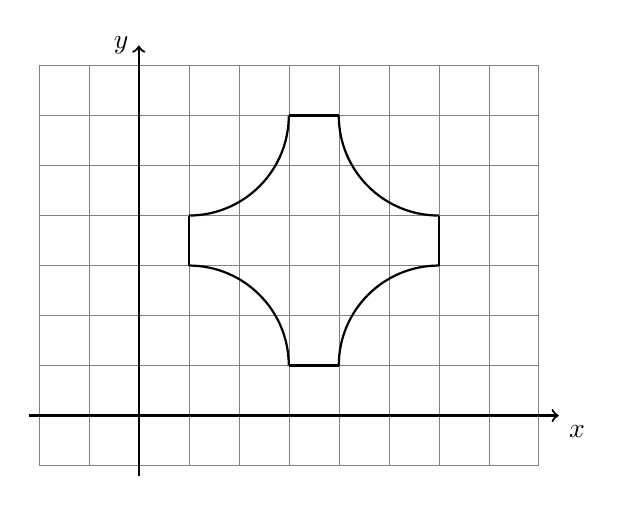
\begin{tikzpicture}[scale=.635]
      \draw [help lines] (-2,-1) grid (8,7);
      \draw [thick, ->] (-2.2,0) -- (8.4,0) node [below right] {$x$};
      \draw [thick, ->] (0,-1.2)--(0,7.4) node [left] {$y$};
      \draw [thick] (6,3)--(6,4);
      \draw [thick] (3,1)--(4,1);
      \draw [thick] (1,3)--(1,4) (3,6)--(4,6);
      \draw [thick] (3,1) arc (0:90:2);
      \draw [thick] (6,3) arc (90:180:2);
      \draw [thick] (6,4) arc (-90:-180:2);
      \draw [thick] (3,6) arc (0:-90:2);
    \end{tikzpicture}
  \end{flushright} \vspace{1cm}
  
  \item Circle $O$ has a radius $AO=7$, as shown below, and $m\angle AOB=72^\circ$.
  \begin{enumerate}
    %\item Find the arc measure $m \wideparen{AB}$. \vspace{1.5cm}
    \item Find the degree measure of the major arc $\wideparen{AB}$.
      \begin{flushright}
      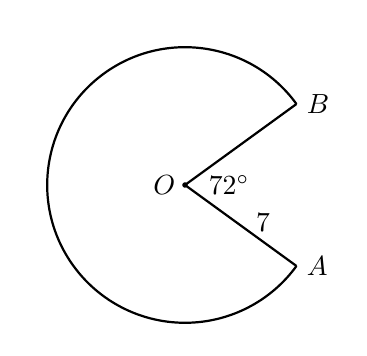
\begin{tikzpicture}[scale=.35]
        %\draw (0,0) circle[radius=5];
        \draw [thick] (36:5) arc (36:324:5);
        \draw [thick] (-36:5) node[right] {$A$}--(0,0);
        \draw [thick] (0,0)--(36:5) node[right] {$B$};
        \fill (0,0) circle[radius=0.1] node[left]{$O$};
        \draw (0:1.6) node{$72^\circ$};
        \draw (-36:3.5) node[above]{$7$};
        %\draw (75:1.8) node[above] {$C$};
        %\draw (290:5) node[below] {$D$};
      \end{tikzpicture}
    \end{flushright}
  \item Find the length of the major arc $\wideparen{AB}$. \vspace{3cm}
  \item Find the area of the figure.
\end{enumerate} \vspace{3cm}

\newpage
\item Which three-dimensional figure will result when a rectangle 6 inches long and 5 inches wide is continuously rotated about the longer side?
    \begin{enumerate}
      \item a rectangular prism with a length of 6 inches, width of 6 inches, and height of 5 inches
      \item a rectangular prism with a length of 6 inches, width of 5 inches, and height of 5 inches
      \item a cylinder with a radius of 5 inches and a height of 6 inches
      \item a cylinder with a radius of 6 inches and a height of 5 inches
    \end{enumerate}

  \item An isosceles right triangle whose legs measure 6 is continuously rotated about one of its legs to form a three-dimensional object. The three-dimensional object is a
    \begin{enumerate}
      \item cylinder with a diameter of 6
      \item cylinder with a diameter of 12
      \item cone with a diameter of 6
      \item cone with a diameter of 12
    \end{enumerate}

  \item A right cylinder is cut perpendicular to its base. The shape of the cross section is a
    \begin{enumerate}
      \item circle
      \item cylinder
      \item rectangle
      \item triangular prism
    \end{enumerate} \vspace{2cm}

  \item A crate in the shape of a rectangular prism must have a volume of 30 cubic feet. It's length is 4 feet and width 3 feet. How tall must it be? \vspace{3.0cm}

\newpage
  \item Randy’s basketball is in the shape of a sphere with a maximum circumference of 29.5 inches. Determine and state the volume of the basketball, to the \emph{nearest cubic inch}. \vspace{4cm}
  
  \item A monument is in the shape of a pyramid with a square base whose sides measure 24 inches and whose height measures 20 feet. What is the volume of the monument, to the \emph{nearest cubic foot}? \vspace{4cm}

  \item A cylindrical pipe with radius $r=6$ inches has a volume of $15.7$ cubic feet. Find the length of the pipe, to the \emph{nearest foot}. \vspace{4cm}

  \item A weather balloon in the shape of a sphere has a volume of $7250$ cubic feet. Find the \emph{diameter} of the balloon, to the \emph{nearest foot}. \vspace{3.5cm}
  

\newpage
  \item A staircase riser is cut as a series of congruent triangles with each step's ``rise" equal to 8 inches, and the ``run" of each step is 10 inches, as shown below in a diagram, \emph{drawn to scale}. ($AB=8$ and $BC=10$) Find the diagonal length of the two-step riser, the distance $AE$, to the \emph{nearest inch}.\\[0.5cm]
        \begin{tikzpicture}[scale=0.5]
          \draw [thick]
          (0,0)node[left]{$A$}--
          (0,8)node[above left]{$B$}--
          (10,8)node[below right]{$C$}--
          (10,16)node[left]{$D$}--
          (20,16)node[right]{$E$}--cycle;
          \draw [dashed, ->] (0,0)--(15,0);
          \draw (0,8)++(0,-0.8)--++(0.8,0)--+(0,0.8);
          \draw (10,16)++(0,-0.8)--++(0.8,0)--+(0,0.8);
          \node at (0,4)[left]{$8$};
          \node at (5,8)[above]{$10$};
          \node at (28:1.5)[right]{$x$};
        \end{tikzpicture}\\
      What is the angle of inclination of the staircase, $x$?
\vspace{1cm}

  \item A bakery sells hollow chocolate spheres. The larger diameter of each sphere is 4 cm. The thickness of the chocolate of each sphere is 0.5 cm. Determine and state, to the nearest tenth of a cubic centimeter, the amount of chocolate in each hollow sphere.
    \begin{flushright}
    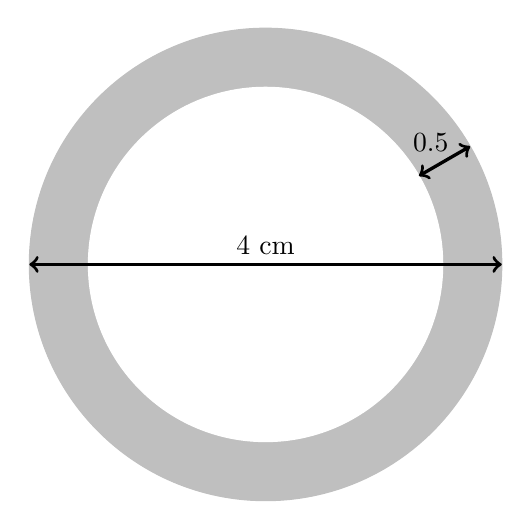
\begin{tikzpicture}[scale=1.5]
      \draw [fill, color=lightgray] (0,0) circle[radius=2];
      \draw [fill, color=white] (0,0) circle[radius=1.5];
      \draw [very thick, <->] (0:2)--(180:2);
      \draw (0,0) node[above]{$4$ cm};
      \draw [very thick, <->]  (30:1.5)--(30:2);
      \draw (32:1.65) node[above]{$0.5$};
    \end{tikzpicture}
    \end{flushright}

\end{enumerate}
\end{document}
